\documentclass[tikz]{standalone}
\usepackage{amsmath}
\usepackage{times}
\usepackage{txfonts}

\usetikzlibrary{arrows}
\usetikzlibrary{intersections}
\usetikzlibrary{math}
\usetikzlibrary{positioning}
\usetikzlibrary{arrows.meta}
\usetikzlibrary{shapes.misc}
\usetikzlibrary{calc}

\begin{document}
  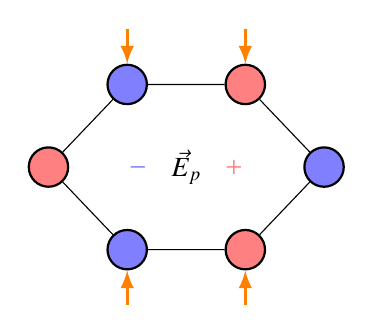
\begin{tikzpicture}[
      >=latex, 
      node distance = 2mm,
      charge/.style = {
        circle, draw = black, thick,
        minimum size = 5mm
      },
      positive/.style = { fill = red!50 },
      negative/.style = { fill = blue!50 },
    ]

    \node[charge, positive, yshift=-2.5mm] (C1) at ( 60:1.5cm) {};
    \node[charge, negative, yshift=-2.5mm] (C2) at (120:1.5cm) {};
    \node[charge, positive, xshift=-2.5mm] (C3) at (180:1.5cm) {};
    \node[charge, negative, yshift= 2.5mm] (C4) at (240:1.5cm) {};
    \node[charge, positive, yshift= 2.5mm] (C5) at (300:1.5cm) {};
    \node[charge, negative, xshift= 2.5mm] (C6) at (360:1.5cm) {};

    \draw[black] (C1) to (C2) to (C3) to (C4) to (C5) to (C6) to (C1);
    % \draw[gray, dashed] (C2) to (C4) to (C6) to (C2);

    \foreach \d in {C1, C2} {
      \draw[orange, very thick, <-] (\d) to ++(0,.7);
    }

    \foreach \d in {C4, C5} {
      \draw[orange, very thick, <-] (\d) to ++(0,-.7);
    }

    \node[black] (E) {\(\vec{E}_p\)};
    \begin{scope}[node distance = .5mm]
      \node[red!50, right = of E] {\(+\)};
      \node[blue!50, left = of E] {\(-\)};
    \end{scope}
    % \draw[gray, thick, dotted] (E) to ++(0,2);
    % \draw[gray, thick, dotted] (E) to ++(0,-2);
  \end{tikzpicture}
\end{document}
